\documentclass[12pt,letterpaper]{article}
\usepackage[margin=1in]{geometry}
\usepackage[english]{babel}
\usepackage[utf8]{inputenc}
\usepackage{setspace} 
\onehalfspacing % Imposta interlinea a 1.5 (Standard accademico)
%\doublespacing % Usa questo se vuoi interlinea doppia (2.0)


\usepackage{amsmath}
\usepackage{amssymb} 
\usepackage[retainorgcmds]{IEEEtrantools}
\usepackage{graphicx}
\usepackage{tabularx}
\usepackage{subfig}
\usepackage{mathptmx} % Times New Roman for text and math
\usepackage{microtype} 
\usepackage{booktabs}   % for nice tables
\usepackage{bm}         % for bold math
\usepackage{listings}   % for inserting code
\usepackage{verbatim}   % useful for program listings
\usepackage{color}  
\usepackage[colorlinks=true, citecolor=blue, linkcolor=black, urlcolor=blue, linkcolor=red]{hyperref} % for blue citations

% use for hypertext
\usepackage[colorinlistoftodos]{todonotes}
\usepackage{natbib}



\begin{document}

%+Title
\title{\textbf{An HANK model and Spending Multipliers: News From a Non Linear World}\\{\small \textbf{Public Economics; \\ University of Bonn ERASMUS+  University of Padova}}}
\author{Lorenzo Del Col}
\date{March 20th, 2026}
\maketitle
%-Title


%+Abstract
\begin{abstract}
This project investigates the transmission mechanism of government spending multipliers under different tax progressivity regimes. Extending the framework of \cite{FN}, we estimate state-dependent multipliers using a Smooth Transition Instrumental Variable Local Projection (STLP-IV) model on U.S. historical data (1913–2006). We confirm the authors' central finding: when identifying fiscal shocks via the News channel \cite{RameyZubairy2018}, the fiscal multiplier is significantly larger (approx. 2.7) when spending is financed by progressive taxes. However, we document a critical sensitivity: this regime dependence disappears when using unanticipated "Surprise" shocks (orthogonalized \cite{BP}). These findings suggest that the "Progressivity Channel" is not mechanical; it relies on an Expectations Channel, where households require the foresight provided by news shocks to adjust their behaviour in response to the distributional tax profile.

\end{abstract}
%-Abstract


\section{Introduction}
Government spending is frequently used to mitigate the effects of recessions. Despite the recurrence of these types of policies the size of the fiscal multiplier remains one of the most debated topics in macroeconomics.
\\
Traditional Keynesian (IS-LM-AS) models usually have large multipliers since the size is given by $Multiplier = \frac{1}{1 - MPC}$ where MPC is the Marginal Propensity to Consume. The multiplier can vary from relatively large to relatively small if the slope of the AS if there is a change from to flat to steep.

In contrast, a spending shock in modern business cycles models usually leads to large crowding out of private consumption in recessions and expansions, hence, the corresponding size of the multiplier is typically around the unity level, way lower than in the Old Keynesian framework. But, when the economy binds the Zero Lower Bound (ZLB) on nominal interest rates, the corresponding multiplier can be larger than unity, as an increase in spending have no effects on interest rates and thus there is no crowding out of investments or consumption \cite{Auerbach_Gorodnichenko_2012_Measuring}.


While early empirical work focused on linear estimates—finding multipliers often below unity \cite{RameyShapiro98, Ramey2011} or larger than unity \cite{BP}—recent literature has shifted toward state-dependent non-linearities. Researchers have questioned whether spending is more effective during recessions \citep{Auerbach_Gorodnichenko_2012_Measuring, CaggianoCastelnuovo_NonLinear, RameyZubairy2018}, when monetary policy is constrained at the Zero Lower Bound, or, crucially for this analysis, when agents possess tax foresight \citep{Ascari}.

%This debate exist is still open also in theoretical works, typically neoclassical and New Keynesian models generate small multipliers, and these results depend heavily on the model specification. The crucial element in theoretical frameworks is the nature of government's budget adjustments to finance the increase in spending \cite{Ohanian1997,Uhlig2010}.

\cite{FN} propose a novel dimension of state dependency: Tax Progressivity.
\\
In their view the distribution across households of the fiscal burden consequent to the stimulus has been neglected in the most HANK literature.
They argue that how the spending is financed matters as much as the spending itself. 
\\
\cite{FN} developed a HANK model to analyze how the distribution of taxes across households shapes spending multipliers.
The model yields empirically realistic distributions in Marginal Propensities to Consume and Labour Participation Elasticities, which result in lower responsiveness to tax changers for higher income earners.
\\
By looking at the historical dimension, on average, U.S. spending shocks were financed with higher tax progressivity.
But not every financing strategies were equal: wars like WWI, WWII, and Korea were financed by progressive tax reforms targeting high-income earners, whereas the Vietnam War and the Reagan defense buildup relied on proportional or regressive financing. The existance of historical variation in financing spending shocks allowed \cite{FN} to empirically test their results coming from the theoretical model, for doing so they estimated a progressivity dependent multiplier.



\subsection{Research Question}
While \cite{FN} provide robust evidence using News shocks (anticipated spending), it remains an open question whether this mechanism holds for all types of fiscal interventions. Recent work by \cite{Ascari} suggests that Tax Foresight—the ability of agents to anticipate future tax liabilities—is crucial for fiscal transmission.

This project asks: Is the Progressivity Multiplier a general feature of fiscal policy, or does it depend on the information set of the agents?

    Specifically, I investigate whether the high multipliers observed under progressive regimes persist when the spending shock is unanticipated, a Surprise shock. Using a Smooth Transition Instrumental Variable Local Projection (STLP-IV) approach, I test the sensitivity of the progressivity channel to three different identification strategies: the \cite{RameyZubairy2018} News shock, with an orthogonalized \cite{BP} Surprise shock, and with an Optimal Instrument that combines both shocks.




\section{Theoretical Framework}
\cite{FN} created an HANK model to analyze how the distribution of taxes shapes spending multipliers. They exploit this by having a rich cross-sectional heterogeneity in marginal propensities to consume and labour supply elasticities which results in lower responsiveness to tax changers for higher-income earners.
\\ 
They find that implied multipliers are larger when spending is financed which an increase in tax progressivity, hence, spending is more expansionary when the tax burden falls more heavily on the higher-income earners.
\\
In the model's environment higher-income earners have exceptional labour market prospects ad thus they face a large opportunity cost of exing the labour market; for this reason the exhibit lower Labour Participation Elasticities, from now on (LPE).
In addition, high discount factor households accumulate more wealth, are often further from their borrowing limits, they have lower Marginal Propensity to Consume (MPC).

\cite{FN} finds that this heterogeneity in the LPE and MPC explains how the distribution of taxes shapes spending multipliers.
That is; a government will rise taxes to finance an increase in spending, and higher taxes crowd out the private sector, which limits how expansionary spending can be. 
Concentrating the higer taxes on the less responsive households, the higher-income ones, reduces the crowding-out effect, in turn increases spending multipliers.

Shifting taxes from the high-MPC to the low-MPC households boosts aggregate demand and thus increase multipliers \cite{FN}.
Heterogeneity in LPE is also important as concentrating taxes on low-LPE workers reduces the crowding-out effect on labour supply, then in consumption.



\subsection{HANK Model}
The Heterogeneous Agent New Keynesian (HANK) framework developed by \cite{FN} introduces heterogeneity in discount factors and an extensive labour supply decision, which result in cross-sectional distribution of Labour Participation Elasticities and Marginal Propensity to Consume . This rich modeling of household decisions is key to understanding how fiscal multipliers depend on the distribution of taxes.
\\
\subsubsection{The HANK Enviroment}
The model is set in discrete time, indexed by $t = 1,2,...$. The economy consists of heterogeneous households, trade unions, intermediate-good producers, a labuor packer, a final-good producer, financial intermediaries, and Fiscal and Monetary authorities.

Households deposit their savings with financial intermediaries and supply hours worked to labour unions. The labour unions combine households' hours into labour services, which they sell to a labour packer. Unions operate under monopolistic competition and face wage adjustment costs \cite{Rotemberg1982}. Intermediate-good producers rent capital and labour to produce outputs sold to a final-good producer, facing similar pricing frictions.

\subsubsection{The Household's Problem}
We focus here on the household problem, which is the primary driver of the transmission mechanism. Let $V_t (a,x,\beta)$ be the value function in period $t$ for a household with assets $a$, idiosyncratic productivity $x$, and discount factor $\beta$. The household solves:

\begin{equation}
    V_t(a,x,\beta) = \max_{c,h,a^\prime} \left\{ \log(c) - B h + \beta \mathbb{E}_t [V_{t+1}(a^\prime,x^\prime,\beta^\prime)] \right\}
    \label{eq:value_function}
\end{equation}

subject to the budget constraint:

\begin{equation}
    c + a^\prime \leq w^h_t x h + (1 + r_t)a - \mathcal{T}_t(w^h_t x h, r_t a) + Z_t + d^h_t(x)
\end{equation}
\begin{equation}
    h \in \{ 0, \bar{h} \}, \quad a^\prime \geq 0
\end{equation}

where $c$ and $h$ denote consumption and hours worked, $w^h_t$ denotes wages perceived by households, and $r_t$ denote the real return on households’ savings. 
Households face a distortionary tax $\mathcal{T}_t(\cdot) \xrightarrow{} Tt(w^h_txh,r_ta)$ which
depends on labour income $w^h_txh$ and capital earnings $r_ta$—and receive a lump-sum transfer $T:t$. Finally, $d^h_t(x)$ represents the dividend payments received from firms.

\subsection{Fiscal Authority and the Tax Function}
The government faces the following budget constraint:

\begin{equation}
    G_t + (1+r^g_t) D_t + Z_t = D_{t+1} + \int \mathcal{T}_t (w_t x h, r_t a) d\mu_t(a,x,\beta)
    \label{eq:gov_budget}
\end{equation}

where $D_t$ is government debt and $G_t$ is government spending.

\subsubsection{Defining Progressivity}
Following \cite{heathcote2017}, the tax function is modeled as $\mathcal{T}_t = \tau_k r a + \mathcal{T}^{lab}_t(y_l)$, where capital income is taxed at a flat rate $\tau_k$, and labour income $y_l$ is taxed according to a non-linear schedule:

\begin{equation}
    \tau^{lab}_t(y_l) = 1 - \lambda_t y_l^{-\gamma_t}
    \label{eq:hsv_tax}
\end{equation}

For the Labour tax they assume a log-linear tax on labour income $y_l$ as $\tau_l(y_l) = 1 - \lambda y^{-\gamma}_l$. With only two parameters, this tax function feautures a remarkable fit to the U.S. federal income tax system:
\begin{itemize}
    \item $\gamma_t$: Controls the \textbf{progressivity} of the tax scheme, describe the level of progressiveness (regressiveness).
    \begin{itemize}
        \item If $\gamma = 0$, the tax rate is flat (constant).
        \item If $\gamma > 0$, the tax function implies a complete redistribution; after-tax labour income $y_l(1 - \tau_l(y_l)) = \lambda$ for any pre-tax income $y_t$. Hence the marginal tax rate increases with income (Progressive).
    \end{itemize}
    \item $\lambda_t$: Controls the \textbf{level} of taxation (revenue). A decrease in $\lambda$ raises the average tax rate for all agents. When $\gamma = 0 $, the tax rate is flat at exactly $1 - \lambda$, hence, an increase in $1 - \lambda$ rises tax rates for all levels of income, while an increase in $\gamma$ makes tax rates higher for high-income and lower for lower-income households.
\end{itemize}


\subsection{Heterogeneity in MPC and LPE}
The model features two dimensions of heterogeneity that are quantitatively critical for the fiscal multiplier.

\paragraph{Marginal Propensity to Consume (MPC):}
Consistent with the empirical literature, the model generates a distribution where MPC declines with liquid wealth. Low-wealth households are often hand-to-mouth consumers with an MPC near 1 \cite{LSEbook}, while wealthy households have an MPC near 0. The average MPC in the model is calibrated by \cite{FN} to approx. 0.16, rising to 0.57 for the lowest wealth quintile.

\paragraph{Labour Participation Elasticity (LPE):}
Labour supply responsiveness is modeled primarily through the extensive margin \citep{Heckman1993}, defined as the discrete decision of whether to participate in the labour market. This choice is particularly relevant for households at the lower end of the wealth distribution—often secondary earners or women—who face significant fixed costs such as childcare, elderly care, or commuting \citep{LSEbook}. Because these agents operate close to the margin of indifference; balancing wages against the fixed disutility of work, their labour supply is highly elastic to tax changes.

In contrast, high-income earners derive a large surplus from employment and exhibit a very low extensive margin elasticity. As documented by \cite{Blundell1995}, these wealthier households are more likely to adjust along the intensive margin varying the number of hours worked, rather than withdrawing from the workforce entirely. Consequently, the LPE is significantly larger for lower-income earners than for those at the top of the distribution.
\\
This is crucially relevant, as the argument \cite{FN} is that financing spending through progressive taxes is more efficient because it targets the high-income group, those with low LPE and low MPC.
These two dimensions of heterogeneity are quantitatively important for the effects of the distribution of taxes on spending multipliers.


\section{Analytical Results: The Transmission Mechanism}

How do these heterogeneities shape the multiplier?  \cite{FN} formalize the transmission mechanism by deriving analytical expressions that link the aggregate effects of fiscal policy to the distribution of taxes. They show that the size of the fiscal multiplier is determined by the covariance between the tax burden and household responsiveness.

\subsection{Tax Effect on Labour Supply ($dL$)}
The authors demonstrate that the aggregate labour supply response ($dL$) to a tax change depends on the distribution of labour supply elasticities. The change in aggregate hours is approximated by the weighted sum of tax rate changes, where the weights are the individual Labour Participation Elasticities:

\begin{equation}
    dL \approx - \int LPE_{i} \times d\tau_{i} d\mu
    \label{eq:labour_response}
\end{equation}

\begin{itemize}
    \item \textbf{Low-Income Households} exhibit a \textbf{high LPE} because they operate on the extensive margin, the decision to participate. A tax increase significantly reduces their probability of working.
    \item \textbf{High-Income Households} exhibit a \textbf{low LPE}. They are inframarginal workers who are unlikely to exit the labour force due to a tax hike.
\end{itemize}

The implication is that a progressive tax shift concentrates the burden on high-income agents (low $\epsilon$), thereby minimizing the aggregate distortion to labour supply ($dL \approx 0$).

\subsection{Tax Effect on Consumption ($dC$)}
Similarly, the aggregate consumption response ($dC$) is linked to the distribution of Marginal Propensities to Consume (MPC):

\begin{equation}
    dC \approx - \int \text{MPC}_{i} \times dT_{i} d\mu
    \label{eq:consumption_response}
\end{equation}

\begin{itemize}
    \item \textbf{Low-Wealth Households} have a \textbf{high MPC}. If taxes reduce their disposable income, they cut consumption almost one-for-one.
    \item \textbf{High-Wealth Households} have a \textbf{low MPC}. They absorb tax increases through lower savings rather than lower consumption.
\end{itemize}

\subsection{Synthesis: The Covariance Channel}
The model predicts that the crowding-out effect is proportional to the covariance between the tax burden and household responsiveness.

\begin{itemize}
    \item \textbf{Non Progressivity (Flat Tax):} Taxes fall on the median agent, creating a positive covariance between the tax burden and responsiveness (High MPC, High LPE), which translates into a large crowding out of both labour and consumption.
    
    \item \textbf{High Progressivity:} Taxes fall on the top earners, creating a zero or negative covariance (Low MPC, Low LPE). This results in a minimal crowding out. The fiscal stimulus boosts demand without triggering a contraction in private spending or labour supply.
\end{itemize}


\section{Spending Multipliers and Tax Progressivity}
Spending is more expansionary when financed with an increase in tax progressivity. While consumption declines in both cases, the contraction is substantially diminished with more progressive taxes. 

Shifting the distribution of taxes across households shapes the aggregate effects of government spending.
\cite{FN} compute the spending multipliers at horizon $h$ for the theoretical model as $m_h = \frac{\sum^{h}_{t=0} (Y_t - Y)}{\sum^{h}_{t=0} (G_t - G)}$ as is typically done in empirical literature, see \cite{RameyZubairy2018, CaggianoCastelnuovo_NonLinear, Auerbach_Gorodnichenko_2012_Measuring}.

The model predicts that government spending is significantly more expansionary when financed with an increase in tax progressivity.
\\
When spending is financed by Non-Progressive taxation, the model generates a multiplier below unity, consistent with standard neoclassical crowding-out effects. However, when the same spending path is financed by a Progressive Tax reform, shifting the burden to high earners, the multiplier increases substantially, often exceeding unity.
\\
By looking at \textcolor{red}{Figure \ref{fig:Figure1FN}, and
\ref{fig:Figure2FN} } we can clearly see that when government spending is financed via a progressive taxation, spending multipliers are larger. This difference in multipliers largely reflects the direct effect of the distribution of taxes.

\subsubsection{Mechanism: Direct vs. Indirect Effects}
To understand the driver of this result, \cite{FN} decompose the aggregate household response into two distinct channels: a Direct Effect stemming from the tax change itself, and an Indirect Effect stemming from general equilibrium price adjustments.

\begin{equation}
    \Delta C_{total} = \underbrace{\Delta C(\text{Taxes})}_{\text{Direct Effect}} + \underbrace{\Delta C(\text{Wages, Dividends})}_{\text{Indirect Effect}}
\end{equation}

The indirect effect captures how households respond to changes in factor prices—specifically, real wages ($w_t$) and interest rates ($r_t$)—induced by the government spending shock.
\begin{itemize}
    \item An increase in $G_t$ raises labour demand, exerting upward pressure on real wages.
    \item Higher wages represent a positive income shock for working households, encouraging higher consumption and labour supply.
\end{itemize}
Crucially, \cite{FN} find that this General Equilibrium effect is remarkably stable across tax regimes. The path of wages and interest rates is similar regardless of how the spending is financed. Thus, the indirect effect provides a baseline boost to the economy in both scenarios.

The divergence in multipliers is driven almost entirely by the direct effect of the tax schedule.

\begin{itemize}
    \item \textbf{Under Low Progressivity:} The tax bill increases for all households, including low-wealth agents with high Marginal Propensity of Consumption (MPC) and high Labour Participation Elasticities (LPE). The negative wealth effect from the tax hike is large enough to overpower the positive wage effect, the net effect is negative, households cut consumption and exit the labour force.

    \item \textbf{Under High Progressivity:} The tax burden is shifted exclusively to high-wealth households.
    \begin{itemize}
        \item \textit{High-Wealth Agents:} They pay the tax but have low MPCs and low LPEs, so their behaviour changes little.
        \item \textit{Median/Low-Wealth Agents:} They experience the positive Indirect Effect (higher wages) without suffering the negative Direct Effect (higher taxes).
    \end{itemize}
    For the median household, the net effect is positive. The crowding-out effect is eliminated, and the aggregate response of consumption and labour is amplified.
\end{itemize}

The reason why there is a difference in the spending multipliers computed under the two different tax regimes lies in the total effect by combining direct and indirect effect of spending shock.
Progressive taxation acts as a shield for the high-MPC population, allowing the expansionary general equilibrium forces,higher wages, to dominate the contractionary partial equilibrium forces, higher taxes.





\section{Empirical Results}
\subsection{The Ferriere and Navarro (2024) Approach}
We explained in depth that the effects of government spending are shaped by the distribution on taxes.
\cite{FN} shows: 
\begin{itemize}
    \item The behaviour of taxes after a spending shock, on average in U.S. history taxes responded proportionally.
    \item They create a non linear spending multiplier.
The datasets covers the period from 1913:Q1 which coincide with the creation of the federal tax system in the U.S., and ends in 2006:Q4.
\end{itemize}

To estimate the Spending Multipliers \cite{FN} use the Local Projection method á la \cite{Jordà2005} combined with an Instrumental Variable approach as \cite{RameyZubairy2018} see also \cite{JordàTaylo2025LP-IV}.

The basic specification is:

\begin{equation}
    \sum^{h}_{j=0} \Delta^j y_{t+h} = \gamma_h + \theta_hZ_t + m_h\sum^{h}_{j=0}\Delta^jg_{t+j} + \varphi trend_t + \epsilon_{t+h}
\end{equation}

Where $\Delta^hy_{t+h} = \frac{Y_{t+h}-Y_{t-1}}{Y_{t-1}}$ is GDP growth, and $\Delta^hg_{t+h} = \frac{G_{t+h}-G_{t-1}}{Y_{t-1}}$ is the adjusted-by-GDP increase in spending, $Z_t$ is the set of controls.
For each horizon $h$, the coefficient $m_t$ measures the cumulative response of output to a $\$1$ increase in governement spending. 
These multipliers has to be interpreted as \cite{Auerbach_Gorodnichenko_2012_Measuring}, they demonstrate by how many dollars GDP increases over time when government spending is increased by $1\$$. 
\cite{FN} use a two stage least square estimator where cumulative spending growth is instrumented by a combination of the \cite{RameyZubairy2018} News Shock, and the \cite{BP} Surprise Shock.
The control matrix $\bm{Z_t}$ include eight lags of GDP, government spending and the average marginal tax rate (AMTR); whereas the trend is quadratic.

In the \cite{FN} linear word, see \textcolor{red}{Figure~\ref{fig:Figure9_Cumulative_Multipliers}} spending induces an output expansion, the multiplier yields a below unity result.


\subsubsection{Progressivity-Dependent Spending Multiplier}

Using this linear specification they estimated and confirmed that the average tax response to a spending shock was progressive.
But is known from the U.S. fiscal history that some war events i.e. Vietnam and Reagan defense buildup, were financed with a low progressive tax reform. 
This historical variation motivates
the focus on how the distribution fn taxes shapes spending multipliers.

The step that \cite{FN} take to pass in the empirical Non-Linear word is building this State-Dependent LP-IV:

\begin{equation}
    \begin{split}
        \sum_{j=0}^{h} \Delta^j y_{t+j} \quad = \quad & \mathbb{I}(p_t = \text{P}) \left\{ \alpha_{P,h} + \bm{A}_{P,h} \bm{Z}_{t-1} + m_{P,h} \sum_{j=0}^{h} \Delta^j g_{t+j} \right\} \\
        & + \mathbb{I}(p_t = \text{N}) \left\{ \alpha_{N,h} + \bm{A}_{N,h} \bm{Z}_{t-1} + m_{N,h} \sum_{j=0}^{h} \Delta^j g_{t+j} \right\} + \phi \, \text{trend}_t + \varepsilon_{t+h}
    \end{split} 
    \label{eq:LP-IV_FN_Model}
\end{equation}




Where, the crucial point is the $p_t$ variable that indicates the state of the word, that is; $P$ when the spending shock is financed via a "Progressive" taxation and the correspondent $N$ for the "Non-Progressive" state.
To identify the state, \cite{FN} created a tax progressivity proxy as a function of  Average Marginal Tax Rat (AMRT) and Average Tax Rate (ATR), that is:

\begin{equation}
    \gamma \equiv (AMTR - ATR)/(1-ATR)
    \label{eq:Gamma_FN}
\end{equation}

The variable $\gamma$ increases when the marginal tax rates increase more than the average tax rate, which often occurs when taxes increase at the top of the income distribution of without largely affecting taxes at the bottom.
\\
The regime is defined as Progressive ($p_t = P$) if the forward-looking average of the progressivity index exceeds its backward-looking average:

\begin{equation}
    p_t = P \quad : \quad \gamma^a_t > \gamma^b_{t-1}
\end{equation}

where the forward-looking average ($\gamma^a_t$) and backward-looking average ($\gamma^b_{t-1}$) are defined respectively as:

\begin{equation}
    \gamma^a_t \equiv \frac{1}{\Delta_a} \sum_{j=0}^{\Delta_a} \gamma_{t+j} \quad \text{and} \quad \gamma^b_{t-1} \equiv \frac{1}{\Delta_b} \sum_{j=1}^{\Delta_b} \gamma_{t-j}
\end{equation}

The remaining quarters are labeled as Non-Progressive ($p_t = N$).
\\
It is important to note that this dummy variable is
ex-post and forward-looking: the classification of a shock at time t depends on the
realization of tax rates at t+1, . . . , t+h. This construction implicitly assumes that agents
have foresight regarding the future financing mix of the fiscal package—a hypothesis that
aligns with ours use of the News shock but may break down under Surprise shocks.


When estimating the Non-Linear multipliers \cite{FN} finds that the effect of government spending on output is significantly larger, but still below unity, for shocks financed with an increase in the progressivity of taxes, see \textcolor{red}{Figure~\ref{fig:Figure14_Progressivity-Dependent_Mult}}. Spending shocks financed via Non-Progressive taxation yields a non significant result.
These empirical results are consistent with their theoretical ones.


\subsection{Identification Strategy - STLP-IV}
Both linear and state dependent IRFs has been estimated in the Fiscal Multipliers literature.
\cite{RameyZubairy2018} used a LP-IV approach, 
some scholars, among others, \cite{Auerbach_Gorodn_2012_FiscalMultil,Auerbach_Gorodnichenko_2012_Measuring, CaggianoCastelnuovo_NonLinear}, Implemented a Smooth Transition VAR (STVAR) approach. More recently \cite{Ascari} implemented a Smooth Transition Local Projection.

Given that \cite{FN} Non-Linear LPs' relies on a dummy variable to switch from the Progressive to the Non-Progressive regime, we think that fiscal reform in response to a spending shock cannot be classified in just these two clusters, we want to allow that the multipliers can be affected by the intensity (Low or High) of progressivity.

For these reasons, we propose an alternative specification and 
estimate the Spending Multiplier on the \cite{FN} dataset by implementing a Smooth Transition Instrumental Variable Local Projections approach (STLP-IV) applying the \cite{GrangerTerasvirtaAnderson1993} Smooth Transition structure combined with LP-IV à la \cite{Jordà2005, JordàTaylo2025LP-IV}.

\subsection{STLP-IV}
We estimate the State-Dependent Impulse Response Functions by projecting the cumulative growth of output on the instrumented government spending shock, allowing coefficients to vary according to the state of the economy. As we are using natural logarithms, this allow us to interpret the estimated coefficients as elasticities, which after are going to be used to retrive the multipliers.
Following \cite{Ascari}, the baseline specification is:

\begin{align}
    y_{t+h} - y_{t-1} & = F(z_{t-1}) \left\{ \alpha^{H}_{h} + \beta^{H}_{h} \text{shock}_t + \bm{A}^{H}_{h} \bm{X}_t \right\} \nonumber \\
    & + (1 - F(z_{t-1})) \left\{ \alpha^{L}_{h} + \beta^{L}_{h} \text{shock}_t + \bm{A}^{L}_{h} \bm{X}_t \right\} + \epsilon_{t+h}
    \label{eq:STLP-IV_BasicModel}
\end{align}
% to call the equation \eqref{eq:STLP-IV_BasicModel}
To be consistent with standard notation in smooth transition literature we need to clarify some change of notation with respect the used one by \cite{FN}.

\begin{itemize}
    \item We call $\bm{X}_t$ the set of controls that \cite{FN} previously called $\bm{Z}_t$
    \item Let $z_t$ the proxy for the Progressive or Non-Progressive state, that is the standardized version of \eqref{eq:Gamma_FN} "$\gamma$" in way to use it in the logistic function.
    \item Let now $\gamma$ be the smoothness parameter of the logistic function. We set $\gamma=3$ calibrated following \cite{Auerbach_Gorodnichenko_2012_Measuring}.
\end{itemize}

Following \cite{GrangerTerasvirtaAnderson1993}, the economy transitions between regimes according to the logistic function $F(z_{t-1})$, bounded between 0 and 1:

\begin{equation}
    F(z_{t-1}) = \frac{\exp(-\gamma z_{t-1})}{1 + \exp(-\gamma z_{t-1})}
    \label{eq:Smooth_Transiction_Function}
\end{equation}

The transition from a state to another is regulated by the standardized transition variable $z_t$. The smoothness parameter $\gamma$ affects the probability of being in a "High-Progressive" regime $F(z_t)$, i.e., the larger the value of $\gamma$, the faster the transition from a state to another. \cite{CaggianoCastelnuovo_NonLinear}.
\\
The Spending Multipliers estimated by a Smooth Transition framework should interpret the reported magnitudes of these multipliers for the two regimes as bounds from polar settings rather than routinely encountered values; more realistic situations will fall between the extremes \cite{Auerbach_Gorodnichenko_2012_Measuring}.

Confidence intervals are computed using the \cite{NeweyWest1987} estimator to account for autocorrelation and heteroskedasticity.

\subsubsection{Calculation of Dollar Multipliers}
Since the coefficients $\beta^H_{h}$ and $\beta^L_{h}$ represent elasticities, we convert them into dollar-equivalent multipliers to make them comparable with the previous literature. We rescale the estimates using the sample average ratio of nominal GDP to Government Spending ($\overline{Y/G}$) as done by \cite{RameyZubairy2018,Auerbach_Gorodnichenko_2012_Measuring,CaggianoCastelnuovo_NonLinear}:

\begin{equation}
    \text{Multiplier}_h = \beta_h \times \frac{\overline{Y}}{\overline{G}}
\end{equation}

This transformation yields the dollar change in GDP resulting from a \$1 change in government spending.

\subsection{Restuls}
As \cite{FN} claims that their LP-IV delivers similar results for both the instruments used in isolation and also when  used in over identification, we want to test these three different specifications with out \eqref{eq:STLP-IV_BasicModel} STLP-IV estimator.
\\
We now present the estimated cumulative multipliers. The central question of this project is whether the "Progressivity Premium" found by \cite{FN} is a general feature of fiscal policy or if it depends on the nature of the shock, Anticipated vs. Unanticipated.

\subsection{Specification 1: The News Channel}
First, we estimate the STLP-IV model using the Anticipated News shock identified by \cite{RameyZubairy2018}. This specification most closely mirrors the baseline analysis in \cite{FN}, but utilizes the smooth transition framework rather than binary dummies.

\textcolor{red}{Figures~\ref{fig:RZ_NonLinear_Multipl_LDC},
\ref{fig:RZ_NonLinear_HighProg_Multipl_LDC}, and \ref{fig:RZ_NonLinear_LowProg_Multipl_LDC} }displays the cumulative dollar multipliers for the High Progressivity (Blue) and Low Progressivity (Red) regimes.

Our results strongly corroborate the findings of \cite{FN}. 
\begin{itemize}
    \item \textbf{High Progressivity:} The multiplier is positive, large, and statistically significant, peaking at approximately 2.7 after 10 quarters.
    \item \textbf{Low Progressivity:} The multiplier is negligible and statistically indistinguishable from zero across all horizons.
\end{itemize}

Unlike the binary classification in \cite{FN}, which averages all episodes above a certain treshold, the smooth transition approach estimates the multiplier at the extreme limit of the transition function $F(z_t) \xrightarrow{}1$.
As noted by \cite{Auerbach_Gorodnichenko_2012_Measuring} these estimates should be interpreted as bounds for a polar settings, representing the theoretical maximum effect of a spending shock financed by an extrimely progressive tax schedule. We interpret the large (2.7) peak of the estimated multiplier in the High-Progressivity state in the ligth of this.
\\
The economic intuition behind this could be that in the polar state, the tax burden on the median household is effectivily zero.
Consequently, the large wealth effect from the government demand shock, higher wages, is not offset by expected taxes, leading to a strong crowding-in of consumption that amplifies the multiplier well above unity. 

This confirms that the STLP estimator captures the same economic dynamics as the \cite{FN} binary model: when the fiscal expansion is anticipated, a progressive financing scheme effectively shields the median agent, preventing the crowding out of consumption.

\subsection{Specification 2: The Surprise Channel}
Does this mechanism persist when agents lack foresight? \textcolor{red}{Figures~\ref{fig:Orth_BP_NonLinear_Multipl_LDC},
\ref{fig:Orth_BP_NonLinear_HighProg_Multipl_LDC}, and \ref{fig:Orth_BP_NonLinear_LowProg_Multipl_LDC} } presents the multipliers estimated using the Orthogonalized Surprise \cite{BP} shock. This shock represents pure surprises, cleaned of any anticipated components.
\\
To ensure a rigorous separation between Anticipated and Unanticipated effects, it is critical that the structural Surprise shock \cite{BP} represents a pure surprise, uncontaminated by the information contained in the News series.

Standard SVAR identification assumes that government spending does not respond to output within the same quarter, but it does not rule out the possibility that spending responds to previously announced plans \citep{Ramey2011}. If the BP shock is correlated with the News shock, the estimates would confound the two transmission mechanisms.

To address this, we clean the BP shock by orthogonalizing it with respect to the \cite{RameyZubairy2018} News variable. 

Following \cite{BP} we retrive the Surprise shock with a trivariate VAR via Cholesky decomposition, with ordering Government Spending first, then GDP and Taxes. This ordering imposes the restriction that government spending does not respond contemporaneously to shocks in output or taxes.

Next, we regress the recovered structural shock $\epsilon^{BP}_t$ on the military news variable:

\begin{equation}
    \epsilon^{BP}_t = \alpha + \delta \text{News}_t + \nu^{OBP}_t
    \label{eq:orthogonalization}
\end{equation}

The residual from this regression, $\nu_t$, captures the variation in government spending that is uncorrelated with the News shock. The estimated orthogonalized series $\hat\nu^{OBP}_t$ serves as the Clean Surprise, the Orthogonlized \cite{BP} instrument in my STLP-IV estimations.

The results point to a crucial divergence. As shown in \textcolor{red}{Figures~\ref{fig:Orth_BP_NonLinear_Multipl_LDC}, and \ref{fig:Orth_BP_NonLinear_HighProg_Multipl_LDC}, and \ref{fig:Orth_BP_NonLinear_LowProg_Multipl_LDC}}:
\begin{itemize}
    \item The point estimates suggest the opposite of the theory, with Low Progressivity yielding slightly higher point estimates.
    \item The regime separation vanishes when taking into account $95\%$ CI bands, the multipliers in the High and Low progressivity states are statistically indistinguishable.
\end{itemize}
This indicates that the Progressivity Premium is not robust to unanticipated shocks. When the spending shock is a surprise, the distribution of taxes appears to be irrelevant for the aggregate transmission.

\subsection{Specification 3: The Optimal Instrument (Over-Identification)}
Finally, I employ an Optimal Instrument approach following \cite{MostlyHarmlessEconometrics}, constructing a first-stage fitted value that combines information from both the News and Surprise shocks.
\\
As displayed in \textcolor{red}{Figures~\ref{fig:Optimal_Instrument_(RZ+BP)_NonLinear_LDC}}, pooling the instruments results in a loss of identification for the progressivity channel. The multipliers in both regimes are low and statistically insignificant at the $95\%$ level. This suggests that the "Surprise" component dominates the variation, washing out the heterogeneity driven by the "News" component.

\section{Conclusion}
This project investigate the transmission mechanism of government spending multiplier under varying regimes of tax progressivity.
\\
Extending the empirical work of \cite{FN}, we employed a Smooth Transition Instrumental Variable Local Projection approach to test whether the progressive premium holds across different identification strategy.
\\
While \cite{FN} argue that "It's All About Taxes," our findings suggest a refinement: "It's All About Expected Taxes." 
\\
Our results confirmed that high tax progressivity boosts fiscal multipliers to a peak of $\approx 2.7$ after $10$ quarters, but only when the spending is anticipated. For unanticipated shocks, the progressivity of the tax code is irrelevant. 
\\
This discrepancy highligths that the transmission mechanism is not mechanical; it relies fundamentally on an expectations channel. As argued by \cite{Ascari}, fiscal foresight changes the information set available to agents, allowing them to adjust their behaviour in anticipation of future policy.

This implies that policymakers aiming to maximize the stimulus effect of progressive taxation must prioritize clear communication and forward guidance to activate the expectations channel.


\clearpage
\bibliographystyle{apalike}
\bibliography{biblio}

%remember to use \citep{} for citation
\section{Replication Files}
\label{app:code}

All econometric estimations, including the construction of the Smooth Transition Local Projection (STLP-IV) estimator and the orthogonalization of the Blanchard-Perotti shock, were performed using \textbf{R}.

To facilitate replication and transparency, the full code and datasets used in this project are hosted on the following GitHub repository:

\begin{center}
    \url{https://github.com/lorenzodelcol99/Public-Economics-Project}
\end{center}

The repository contains:
\begin{itemize}
    \item \texttt{main\_script.R}: The primary script for estimating the non-linear multipliers.
    \item \texttt{Dataset}: The folder contains the dataset provided by the \cite{FN} replication package
    \item \texttt{R\_Images\_LDC}: The folder containing the high-resolution output plots.
\end{itemize}

\section{Apendix}

%FN Images

\begin{figure}
    \centering
    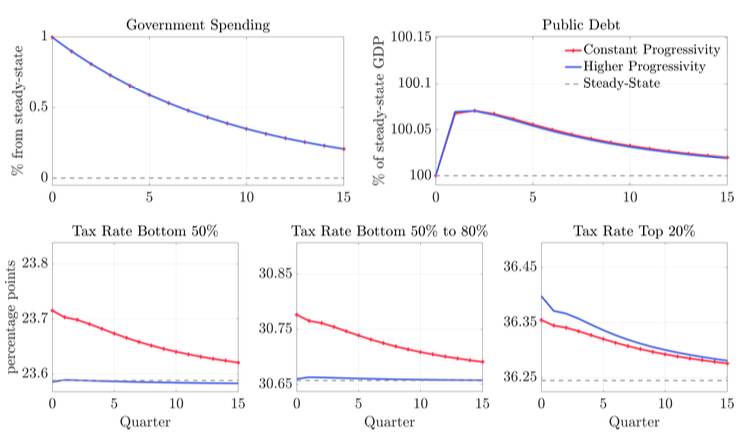
\includegraphics[width=1\linewidth]{FN_Images/Figure1_Spending_Shock.png}
    \caption{Spending Shock Financed with Different Paths for Progressivity: Fiscal Policy. Source: \citep{FN}. }
    \label{fig:Figure1FN}
\end{figure}

\begin{figure}
    \centering
    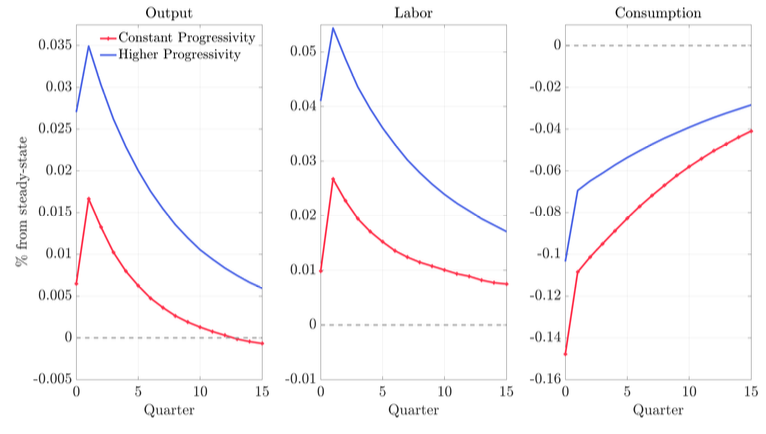
\includegraphics[width=1\linewidth]{FN_Images/Figure2_NonLin_Model_Response.png}
    \caption{Model Responses to a Spending Shock Financed with Different Paths for Progressivity. Source: \citep{FN}.}
    \label{fig:Figure2FN}
\end{figure}

\begin{figure}
    \centering
    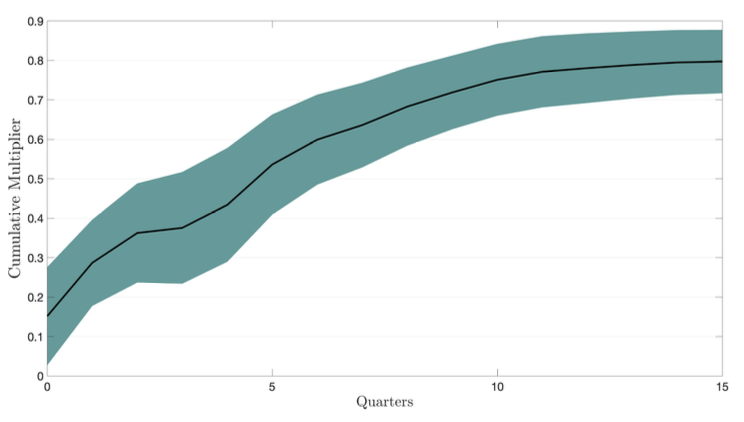
\includegraphics[width=1\linewidth]{FN_Images/Figure9_Cumulative_Multipliers.png}
    \caption{Cumulative Multipliers. 68\% CI level. Source: \citep{FN}.}
    \label{fig:Figure9_Cumulative_Multipliers}
\end{figure}

\begin{figure}
    \centering
    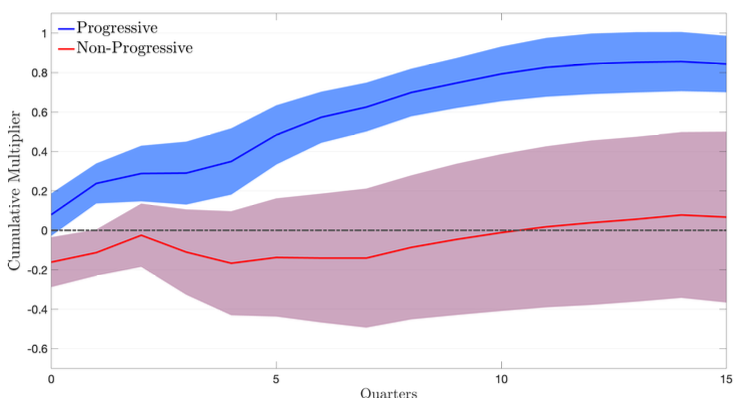
\includegraphics[width=1\linewidth]{FN_Images/Figure14_Progressivity-Dependent_Mult}
    \caption{Progressivity-Dependent Cumulative Multipliers. 68\% CI level. Source: \citep{FN}.}
    \label{fig:Figure14_Progressivity-Dependent_Mult}
\end{figure}

% LDC Images

\begin{figure}
    \centering
    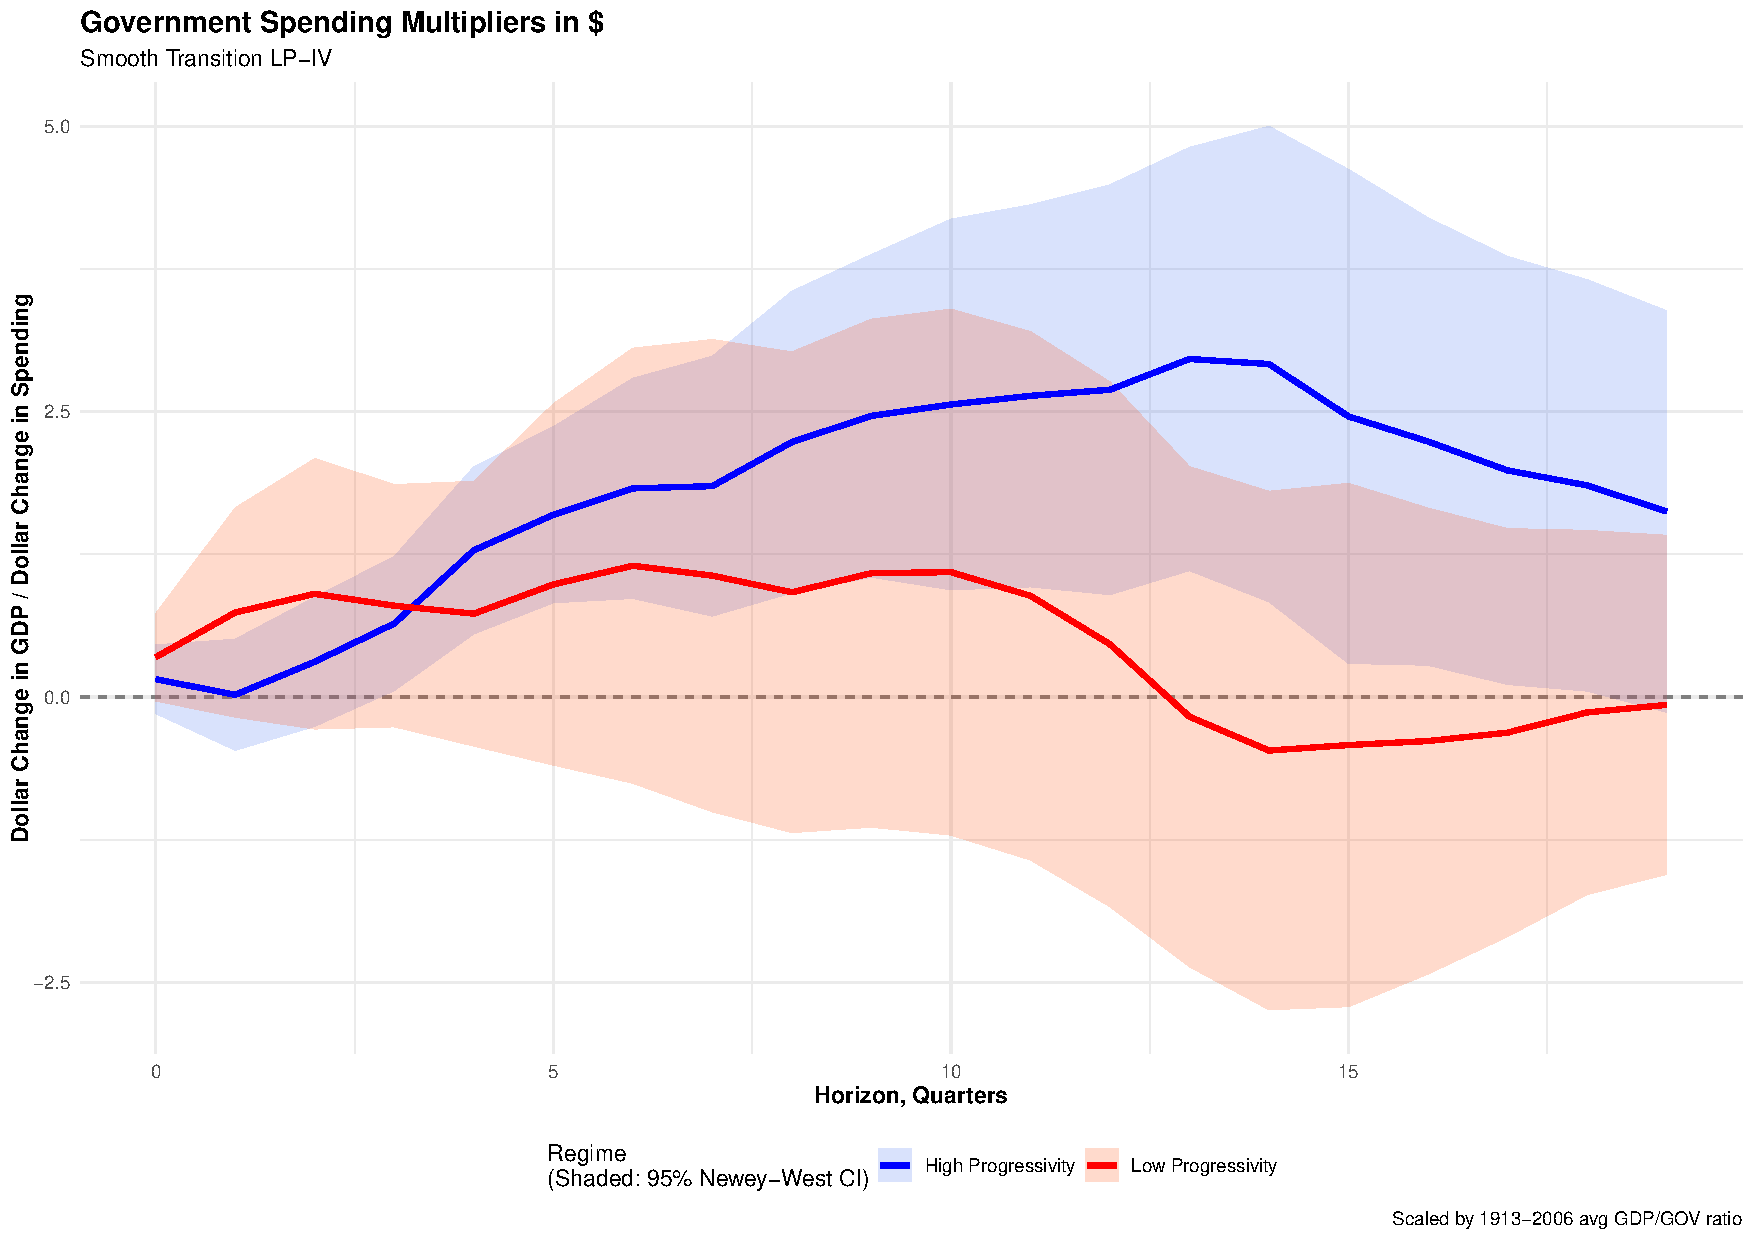
\includegraphics[width=1\linewidth]{R_Images_LDC/RZ_NonLinear_Multipl_LDC.pdf}
    \caption{Non Linear Spending Multiplier estimated by STLP-IV under Just Identification with the NEWS \cite{RameyZubairy2018} Shock}
    \label{fig:RZ_NonLinear_Multipl_LDC}
\end{figure}

\begin{figure}
    \centering
    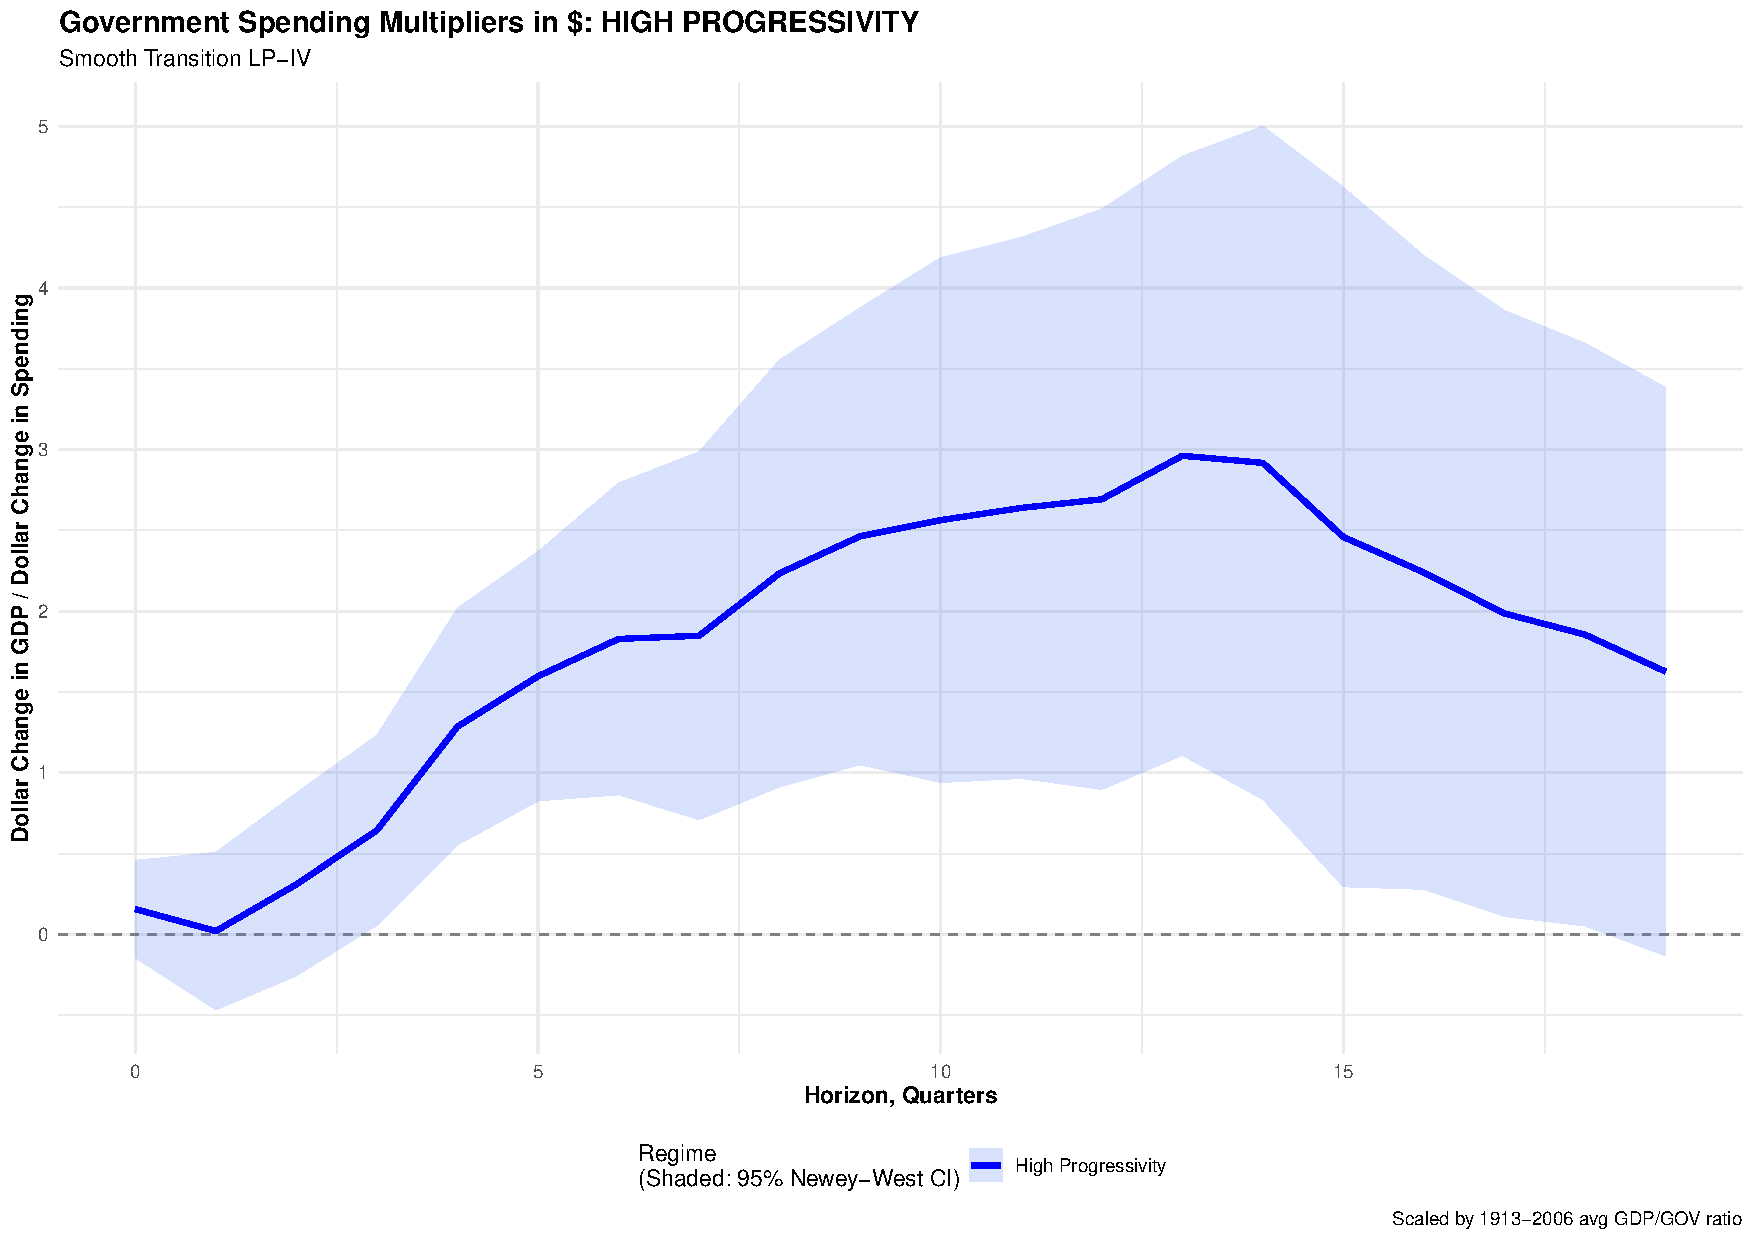
\includegraphics[width=1\linewidth]{R_Images_LDC/RZ_NonLinear_HighProg_Multipl_LDC.pdf}
    \caption{"High-Progressivity" Non Linear Spending Multiplier estimated by STLP-IV under Just Identification with the NEWS \cite{RameyZubairy2018} Shock}
    \label{fig:RZ_NonLinear_HighProg_Multipl_LDC}
\end{figure}

\begin{figure}
    \centering
    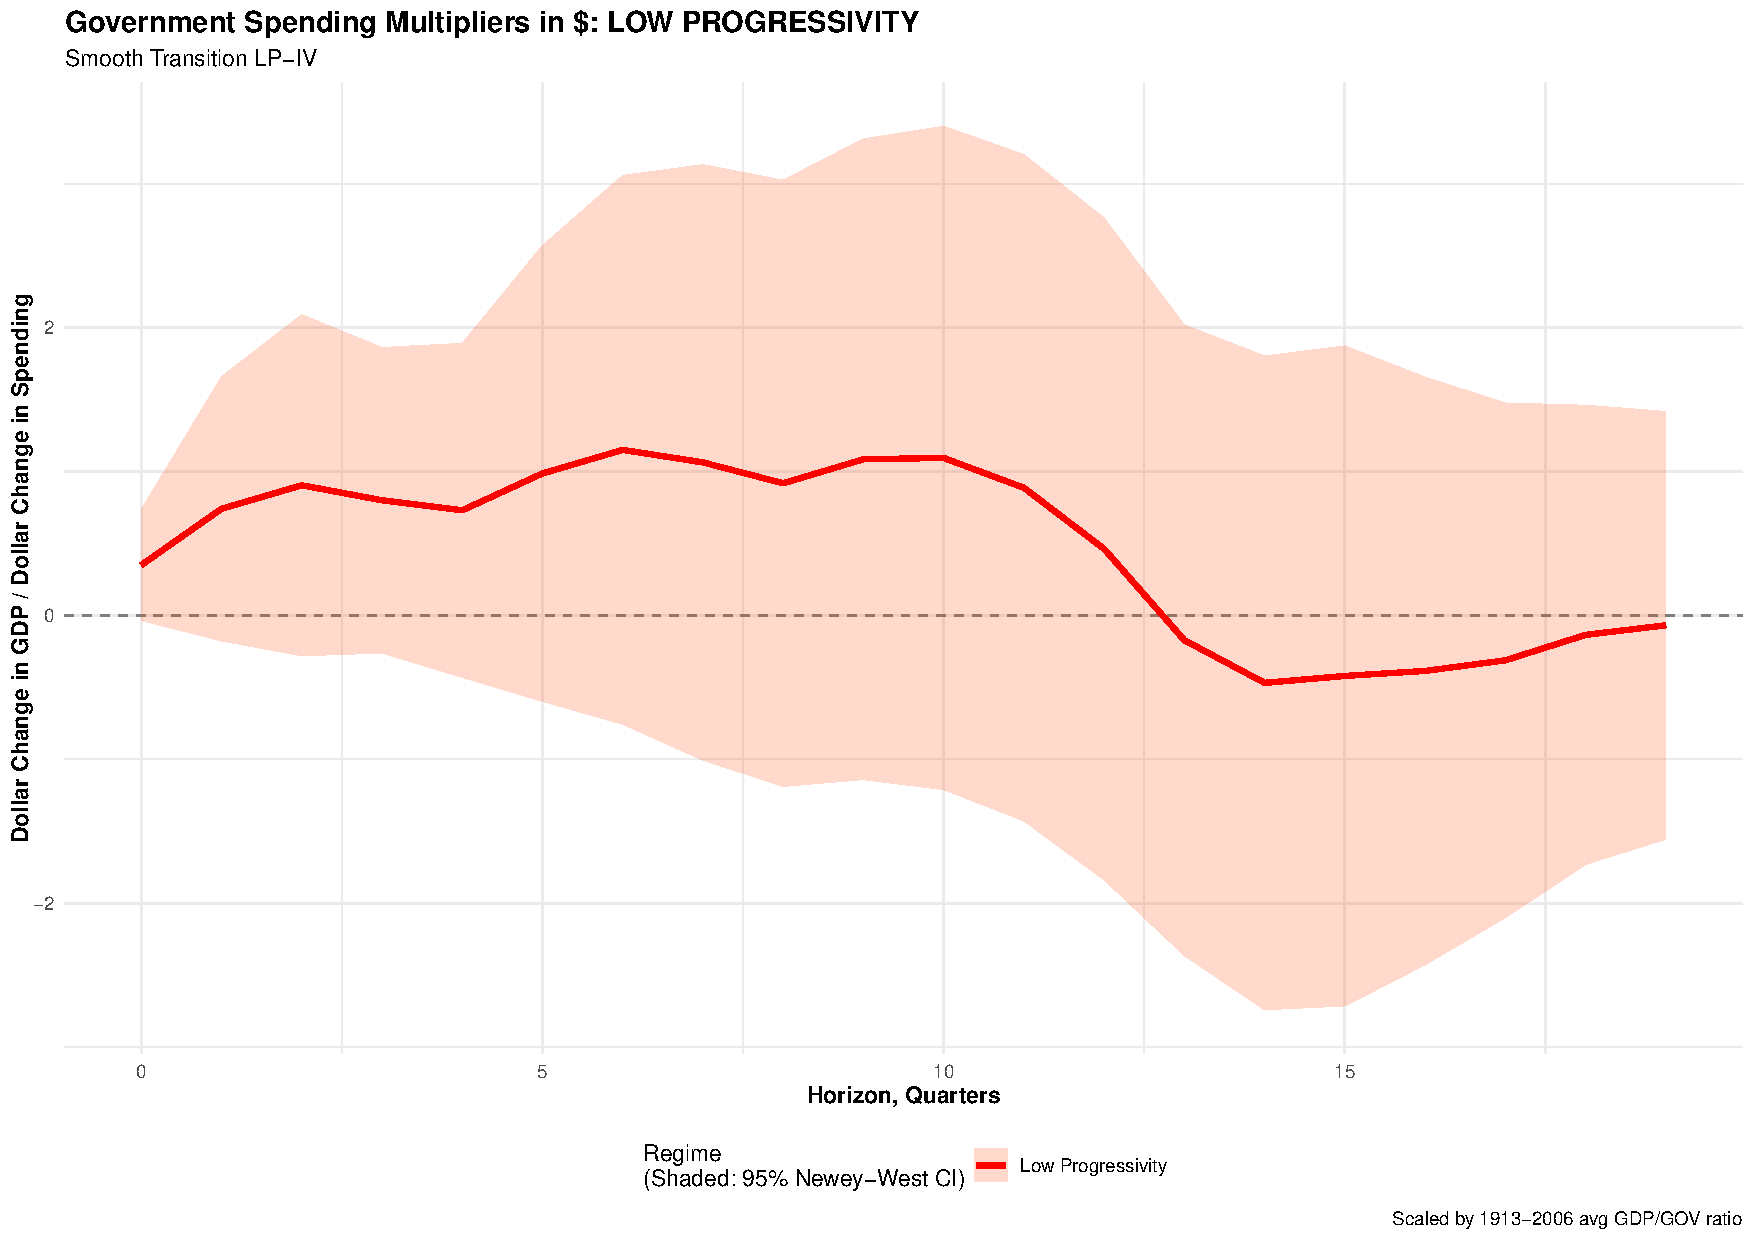
\includegraphics[width=1\linewidth]{R_Images_LDC/RZ_NonLinear_LowProg_Multipl_LDC.pdf}
    \caption{"Low-Progressivity" Non Linear Spending Multiplier estimated by STLP-IV under Just Identification with the NEWS \cite{RameyZubairy2018} Shock}
    \label{fig:RZ_NonLinear_LowProg_Multipl_LDC}
\end{figure}

\begin{figure}
    \centering
    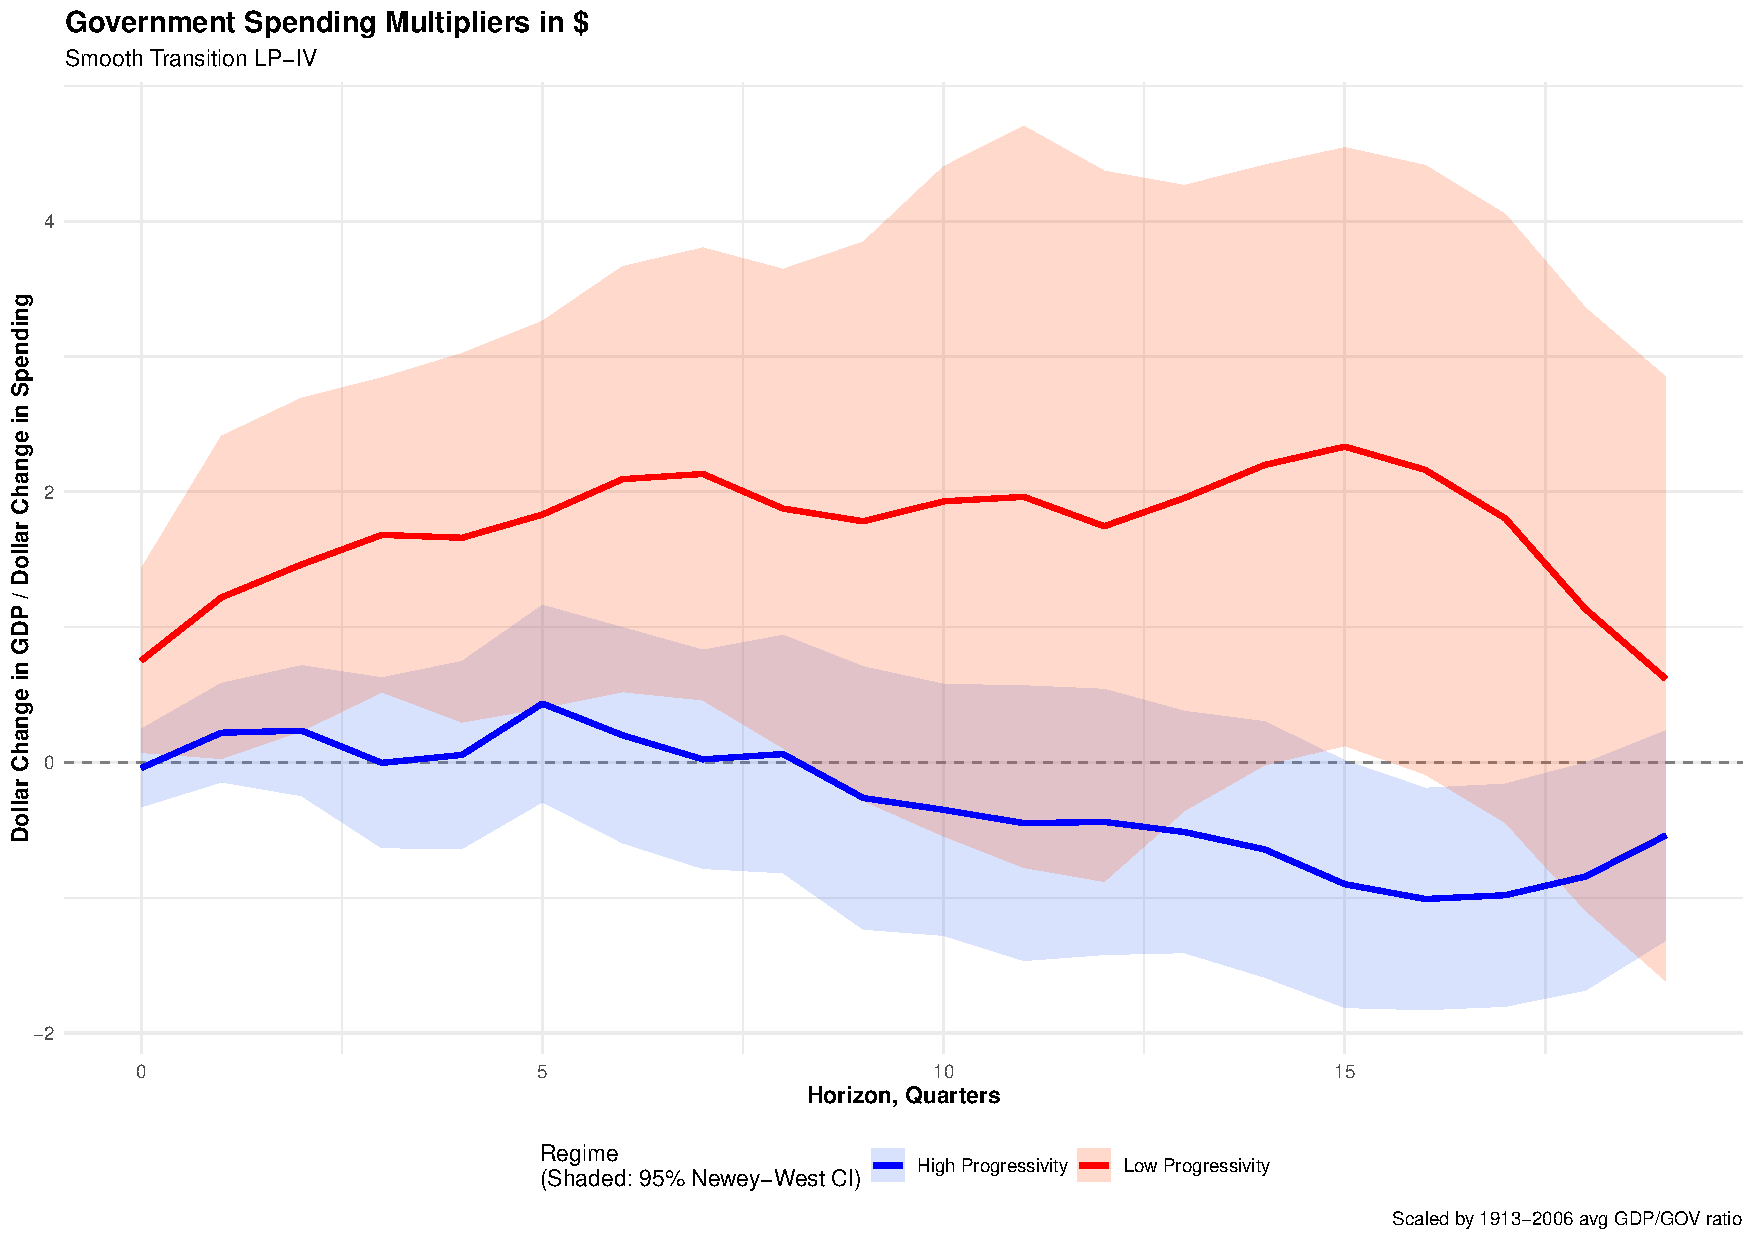
\includegraphics[width=1\linewidth]{R_Images_LDC/Orth_BP_NonLinear_Multipl_LDC.pdf}
    \caption{Non Linear Spending Multiplier estimated by STLP-IV under Just Identification with the Orthogonalized Surprise \cite{BP} Shock}
    \label{fig:Orth_BP_NonLinear_Multipl_LDC}
\end{figure}

\begin{figure}
    \centering
    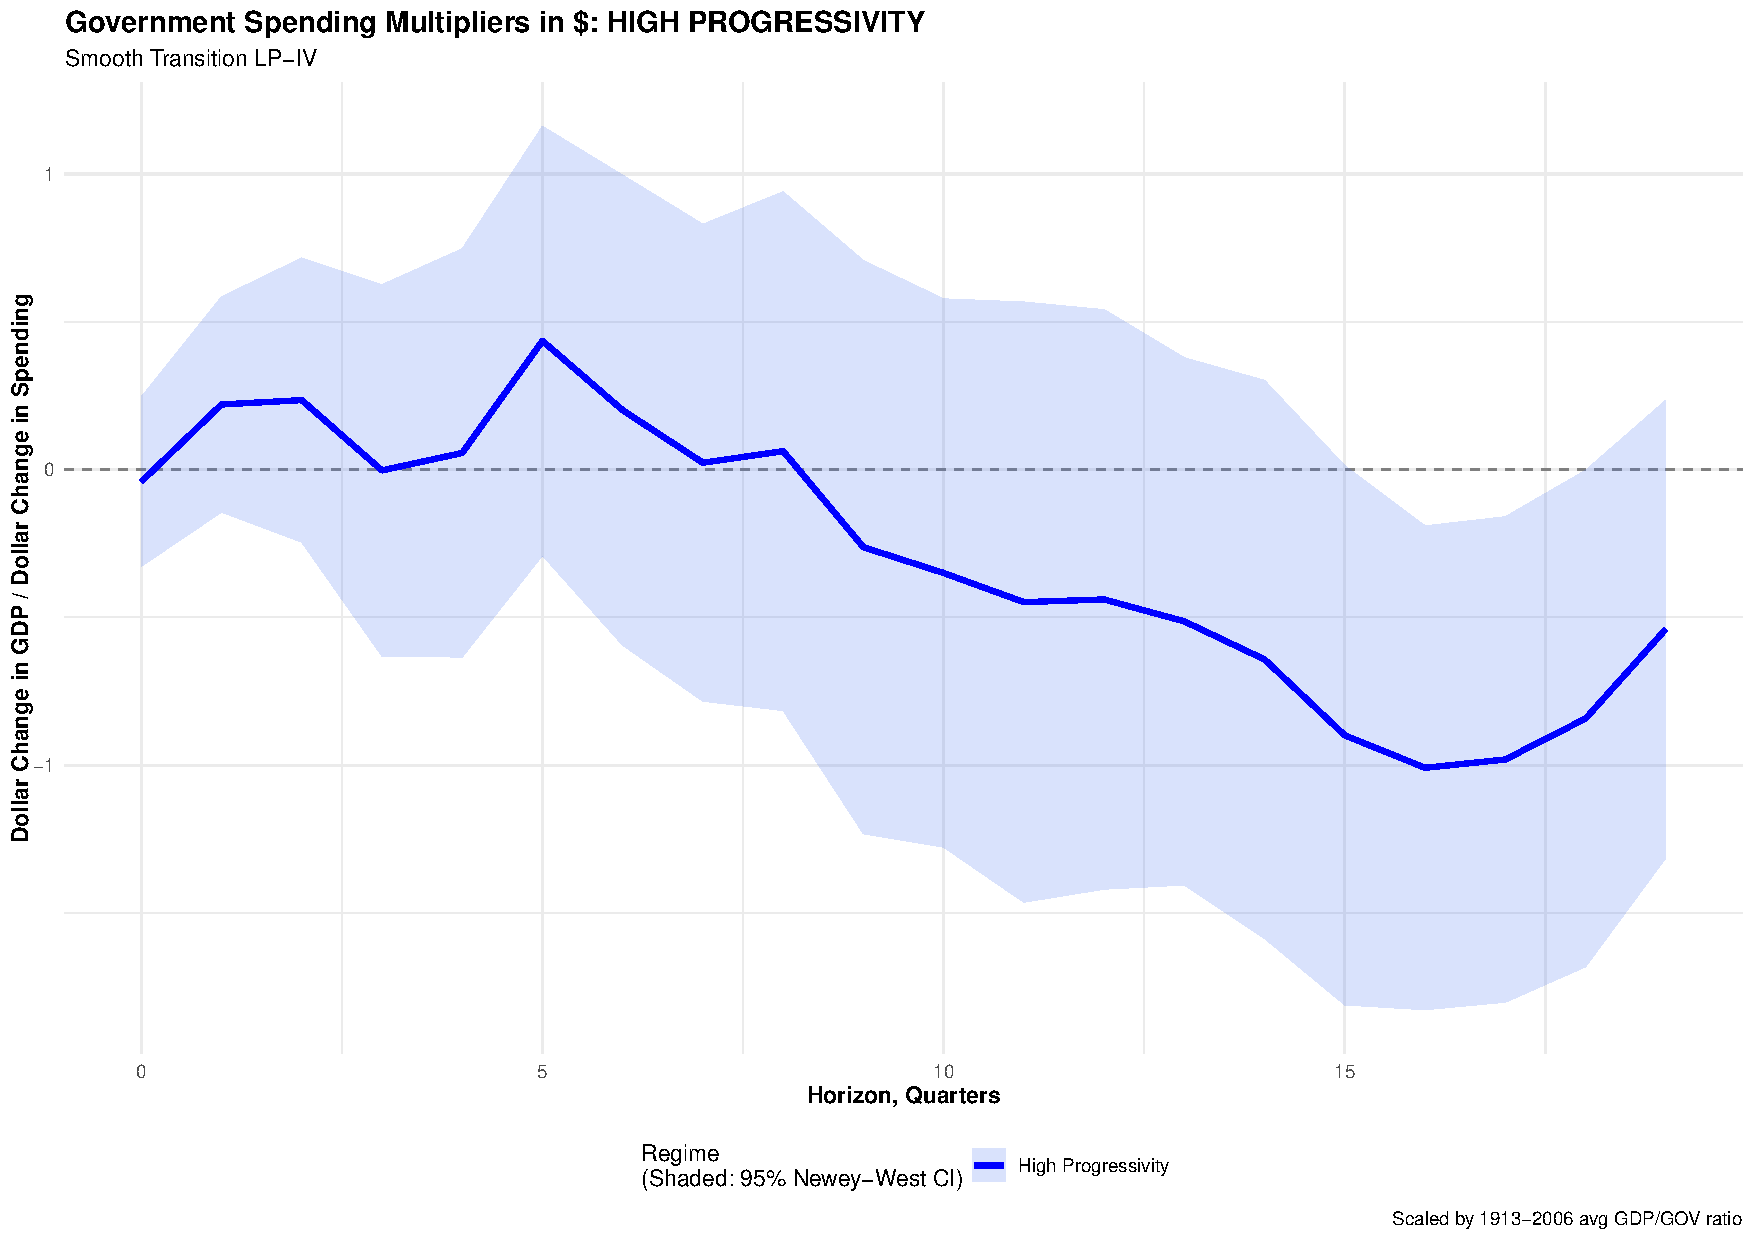
\includegraphics[width=1\linewidth]{R_Images_LDC/Orth_BP_NonLinear_HighProg_Multipl_LDC.pdf}
    \caption{"High-Progressivity" Non Linear Spending Multiplier estimated by STLP-IV under Just Identification with the Orthogonalized Surprise \cite{BP} Shock}
    \label{fig:Orth_BP_NonLinear_HighProg_Multipl_LDC}
\end{figure}

\begin{figure}
    \centering
    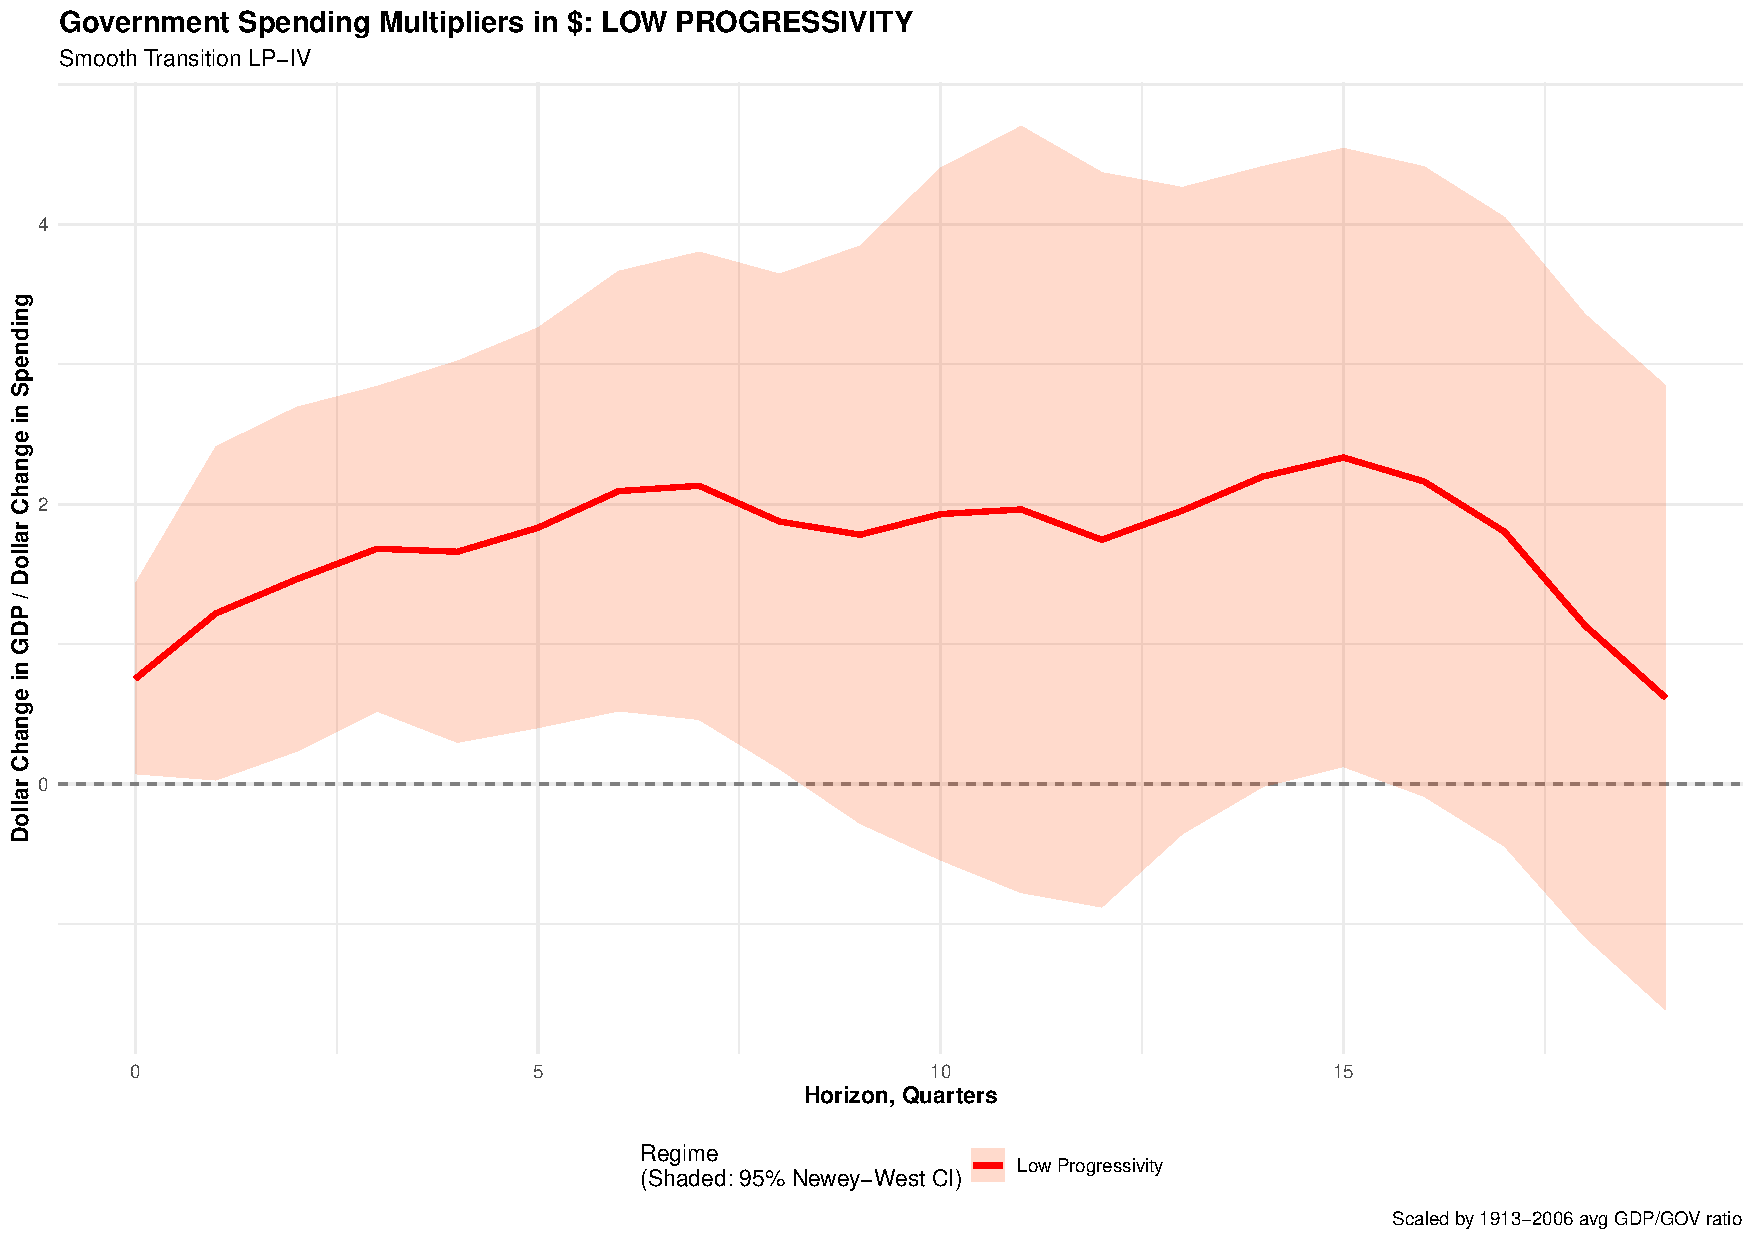
\includegraphics[width=1\linewidth]{R_Images_LDC/Orth_BP_NonLinear_LowProg_Multipl_LDC.pdf}
    \caption{"Low-Progressivity" Non Linear Spending Multiplier estimated by STLP-IV under Just Identification with the Orthogonalized Surprise \cite{BP} Shock}
    \label{fig:Orth_BP_NonLinear_LowProg_Multipl_LDC}
\end{figure}

\begin{figure}
    \centering
    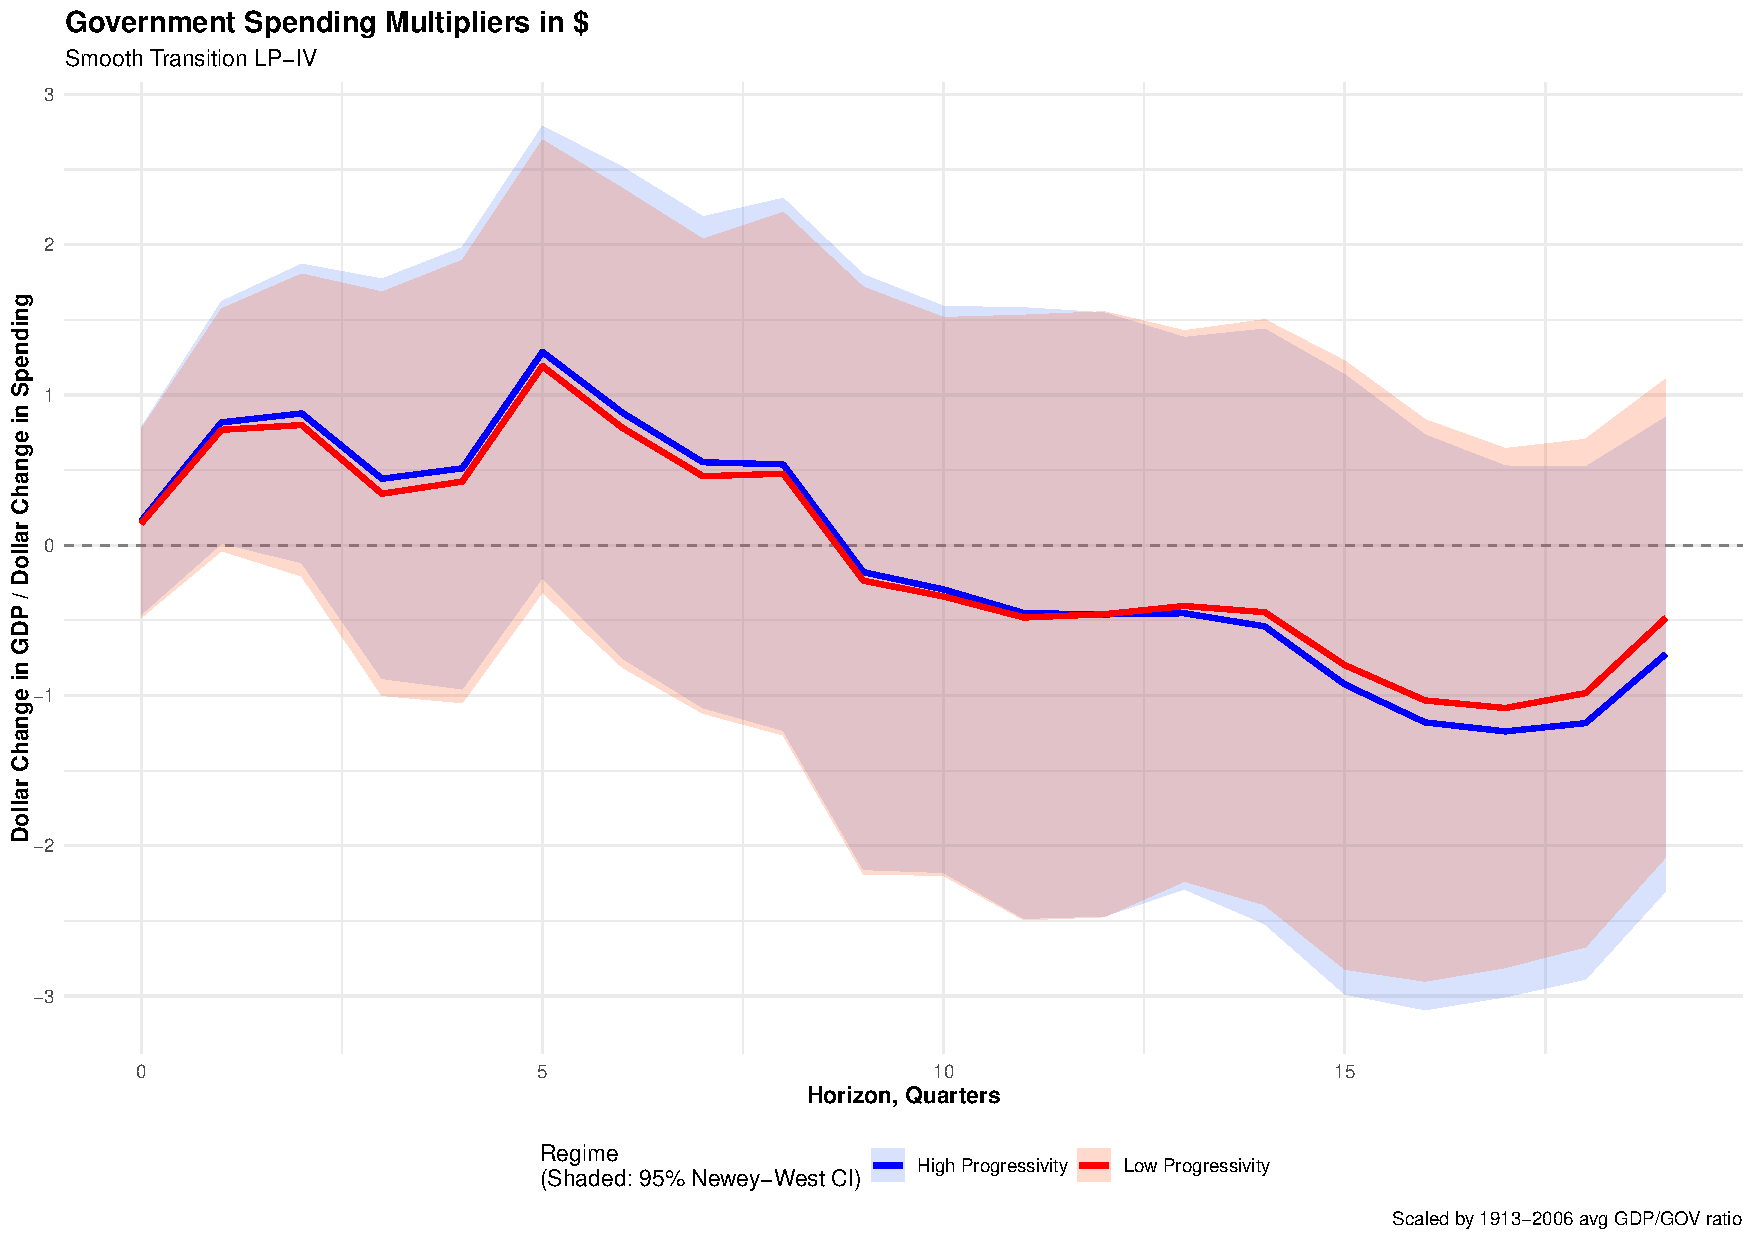
\includegraphics[width=1\linewidth]{R_Images_LDC/Optimal_Instrument_(RZ+BP)_NonLinear_LDC.pdf}
    \caption{Non Linear Spending Multiplier estimated by STLP-IV under Over Identification with the Optimal Instrument composed by the  Orthogonalized \cite{BP} and News \cite{RameyZubairy2018} Shoks}
    \label{fig:Optimal_Instrument_(RZ+BP)_NonLinear_LDC}
\end{figure}

\end{document}